\chapter{Approach}\label{ch:approach}

In this research's scope, we propose our new concurrent range-locking design that leverages a probabilistic concurrent skip list~\parencite{herlihy2006provably, herlihy2020art}.
It consists of two main functions:
\begin{itemize}
    \item \textbf{tryLock}: The \texttt{tryLock} function searches for the required range \texttt{[start,end]} in the skip list.
    If an overlapping range exists, indicating another thread is modifying that range, the requesting thread must wait and retry.
    If not, the range is added to the list, signaling that the range is reserved.
    \item \textbf{releaseLock}: The \texttt{releaseLock} function releases the lock by finding the address range in the skip list and removing it accordingly.
\end{itemize} 

Our range lock design is also lock-free.
It relies on atomic operations (\texttt{compareAndSet()}), thus addressing the bottleneck problem of the spinlock-based range lock and maintaining the lock's high level of performance.

\section{Skip List}\label{sec:skip-list}

A skip list is a probabilistic data structure.
It allows fast search, insertion, and deletion.
It is an alternative to balanced trees, such as AVL trees or red-black trees~\parencite{pugh1990skip, pugh1990skip2}.
The key idea of a skip list is to use multiple layers of sorted linked lists to maintain elements, where each layer is an \("\)express lane\("\) for faster traversal.

\begin{figure}[h]
    \centering
    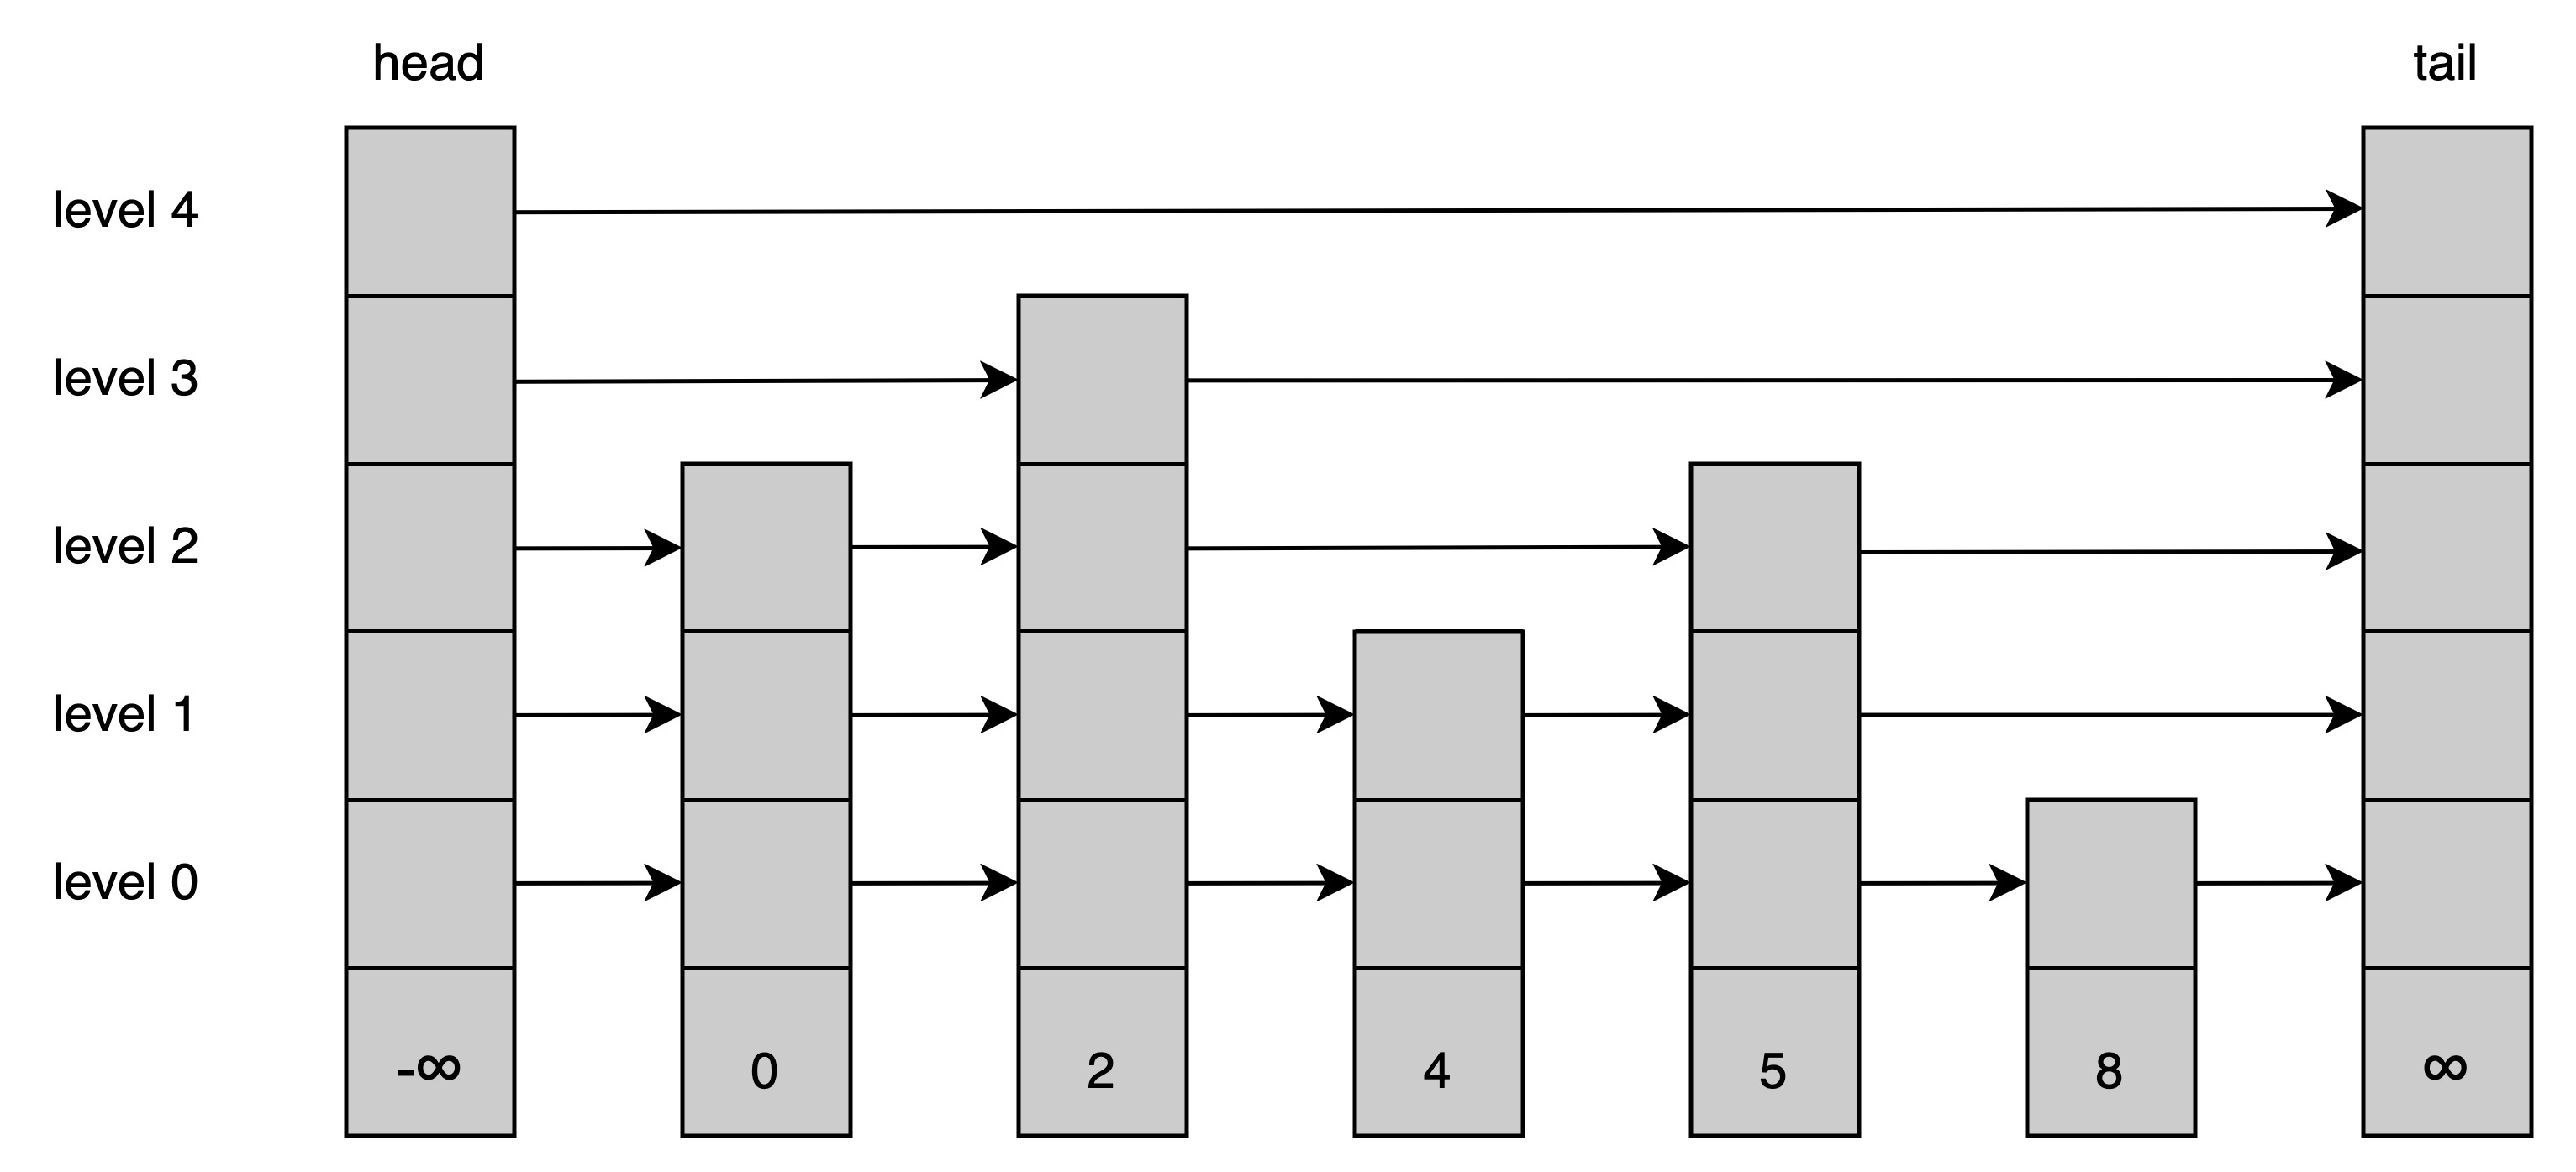
\includegraphics[width=0.8\textwidth]{./figures/skiplist}
    \caption{Skip List: this example has five levels of sorted linked lists. \\
 Each \texttt{Node} has a unique key, and the head and tail have $-\infty$ and $+\infty$ keys.}
    \label{fig:skiplist}
\end{figure}

\subsection*{How it work}

\textbf{Multiple Layers:} A skip list consists of multiple layers where the bottom-most layer is a regular sorted linked-list.
Each higher layer acts as an \("\)express lane\("\) that speeds up access by skipping over multiple elements from the layer below.
Nodes in higher layers provide shortcuts, allowing faster traversal across the list and effectively reducing the time complexity of search operations.

\textbf{Probabilistic Balancing:} Each \texttt{Node} is created with a random top level and belongs to all lists up to that level.
Top levels are chosen so that the expected number of nodes in each level's list decreases exponentially.
Let \(0 < p < 1\) be the conditional probability that a \texttt{Node} at level \(i\) also appears at level \(i + 1\).
All nodes appear at level \(0\).
The probability that a \texttt{Node} at level 0 also appears at level \(i > 0\) is \( p^i\).
For example, with \(p = 1/2\), \(1/2\) of the nodes are expected to appear at level \(1\), \(1/4\) at level 2, and so on, providing a balancing property like the classical sequential tree-based search structures, except without the need for complex global restructuring.
This random generation ensures that the list structure remains balanced.
Consequently, skip list insertion and deletion algorithms are much simpler and faster than equivalent algorithms for balanced trees.

\textbf{Search Operation:} To search for an element, the algorithm starts at the topmost layer and moves horizontally through the elements of that layer.
When it encounters an element greater than the target, it drops to the next lower layer and continues the search horizontally.
This process of horizontal traversal and vertical descent continues until the target element is found or the search reaches the bottom-most layer without finding the target.
The hierarchical structure allows for logarithmic search time.

\textbf{Insertion and Deletion:} Inserting an element involves locating the appropriate position in the bottom-most layer, placing the element there, then potentially promoting the element to higher layers.
Each promotion step is independent, ensuring the probabilistic balancing of the structure.
Deleting an element requires removing it from all layers in which it appears, which is straightforward once the element is located using the search algorithm.
The process of updating references in multiple layers ensures that the skip list remains balanced and efficient for subsequent operations.

\begin{figure}[h]
    \centering
    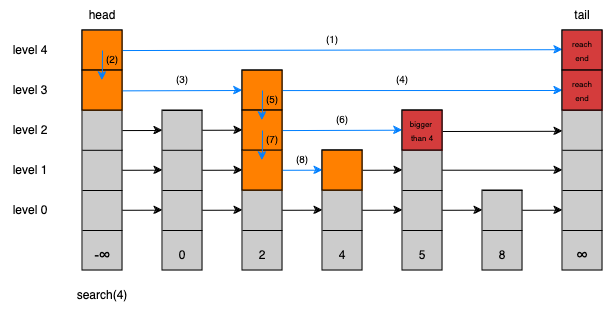
\includegraphics[width=0.8\textwidth]{./figures/skiplistsearch}
    \caption{Skip List: In this example, the list searches for a \texttt{Node} with value 4. It starts on the head \texttt{Node} on the highest level, tries to move horizontally until it reaches a greater value than 4, and then goes down a level and repeats. The number noted on the arrows implies the order of the traversal.}
    \label{fig:skiplistsearch}
\end{figure}

Despite their theoretically poor worst-case performance, skip lists rarely exhibit worst-case behavior, making them efficient in most scenarios.
For instance, in a dictionary with over 250 elements, the likelihood of a search taking more than three times the expected duration is less than one in a million~\parencite{pugh1990skip2}.
Skip lists are ideal for implementing range locks, offering a balanced structure that improves concurrency.

\begin{table}[h!]
    \centering
    \begin{tabular}{|c|c|c|c|}
        \hline
        \textbf{Operation} & \textbf{Best Case} & \textbf{Average Case} & \textbf{Worst Case} \\ \hline
 Search, Insert, Delete & $O(1)$ & $O(\log n)$ & $O(n)$ \\ \hline
    \end{tabular}
    \caption{Time complexities of skip list operations}
    \label{tab:skiplisttimecomplexity}
\end{table}

\newpage

\section{Concurrent Range Lock}\label{sec:concurrent-range-lock}
We developed our concurrent range lock based on the design of \texttt{LockFreeSkipList} proposed by Herlihy et al.~\parencite{herlihy2020art}.
In summary, LockFreeSkipList uses atomic operations (\texttt{compareAndSet()}) to manage \texttt{Node} references without locks, which enhances performance in multithreaded environments.
When adding a \texttt{Node}, the process starts at the lowest level and moves upward to ensure immediate visibility.
Removing a \texttt{Node} involves marking nodes from the top down before unlinking them.
Furthermore, it relaxes strict structural maintenance of higher levels, focusing on the bottom-level list for set representation, which offers improved scalability and efficiency.
We made some modifications to adapt this structure to our concurrent range lock.

For the sake of simplicity, we use uint for our pseudocode provided in this section.
In our open-source C++ implementation, we use the template to enable generic programming.

\subsection{The idea}\label{subsec:the-idea}

The \texttt{ConcurrentRangeLock} class provides a concurrent mechanism to manage range-based locks.
Its primary API includes methods for locking and unlocking ranges.
Each range is stored in a single \texttt{Node}.
The \texttt{tryLock} method attempts to acquire a lock for the specified range \texttt{[start, end]}, returning \texttt{true} on success and \texttt{false} otherwise.
The \texttt{releaseLock} method releases the lock for the range \texttt{[start, end]}, with \texttt{true} indicating success and \texttt{false} if the range was not found or an error occurred.

The two primary methods rely heavily on \texttt{find} methods such as \texttt{findInsert}, \texttt{findExact}, and \texttt{findDelete}, which handle insertion, exact range finding, and deletion of ranges, respectively.

All of these methods will be discussed in section \ldots (ref).

\begin{lstlisting}[style=mystyle, caption=Concurrent Range Lock,label={}]
class ConcurrentRangeLock {
  public:
    ConcurrentRangeLock();

    bool tryLock(uint64_t start, uint64_t end);
    bool releaseLock(uint64_t start, uint64_t end);

  private:
    Node<uint64_t> *head, *tail;
    int randomLevel();

    bool findInsert(uint64_t start, uint64_t end, Node<uint64_t> **preds, Node<uint64_t> **succs);
    bool findExact(uint64_t start, uint64_t end, Node<uint64_t> **preds, Node<uint64_t> **succs);
    void findDelete(uint64_t start, uint64_t end);
};
\end{lstlisting}

\subsection{Node}\label{subsec:node}

We made a critical modification inside the \texttt{Node} structure.
Each \texttt{Node} now contains \textbf{\texttt{start}} and \textbf{\texttt{end}}, instead of \textbf{\texttt{key}} and \textbf{\texttt{value}}, which represent the acquired range associated with the Node.
\texttt{Node} also uses an array of \textbf{\texttt{AtomicMarkableReference}} (more details in section \ref{subsec:atomicmarkablereference}) to maintain forward links at each level, which allows for efficient traversal and updates.
The \texttt{initialize} method sets up a \texttt{Node} with specific range and level values.
In contrast, \textbf{\texttt{initializeHead}} configures the head \texttt{Node} with forward pointers directed to a provided tail \texttt{Node}, establishing the initial structure.
Additionally, the \texttt{Node} class provides accessor methods to retrieve the Node's properties.

\vspace{15pt}

\begin{lstlisting}[style=mystyle, caption=Node class implementation,label={}]
class Node {
  private:
    uint64_t start, end;
    int topLevel;
    AtomicMarkableReference<Node>** next;

  public:
    Node() : next(nullptr) {}

    void initialize(uint64_t start, uint64_t end, int topLevel) {
    this->start = start;
    this->end = end;
    this->topLevel = topLevel;

    next = new AtomicMarkableReference<Node>*[topLevel + 1];
    for (int i = 0; i <= topLevel; ++i)
    next[i] = new AtomicMarkableReference<Node>();
    }

    void initializeHead(uint64_t start, uint64_t end, int topLevel, Node* tail) {
    initialize(start, end, topLevel);
    for (int i = 0; i <= topLevel; ++i)
    next[i]->store(tail, false);
    }

    int getTopLevel() const { return topLevel; }
    uint64_t getStart() const { return start; }
    uint64_t getEnd() const { return end; }
};
\end{lstlisting}

\subsection{AtomicMarkableReference} \label{subsec:atomicmarkablereference}

\texttt{AtomicMarkableReference} is designed to maintains an object reference (in this case \texttt{Node}) along with a mark bit, that can be updated atomically~\parencite{atomicMarkableReference}.

The \texttt{AtomicMarkableReference} class uses a single atomic variable, \texttt{atomicRefMark}, to store a packed representation of the reference and the mark.
These values are packed and unpacked using bitwise operations, where the least significant bit represents the mark.
The class offers several atomic methods:

\begin{itemize} 
    \item \texttt{store}: directly sets the reference and mark.
    \item \texttt{compareAndSet}: tests if the current reference and mark match the expected values and, if so, updates them to new values atomically. 
    \item \texttt{attemptMark}: sets the mark if the reference matches the expected value.
    \item \texttt{get}: returns both the object's reference and sets the mark reference. 
    \item \texttt{getReference}: returns just the reference of the object.
\end{itemize}

\vspace{15pt}
    
\begin{lstlisting}[style=mystyle, caption=AtomicMarkableReference class implementation,label={}]
const uintptr_t MARK_MASK = 0x1;

class AtomicMarkableReference {
  private:
    std::atomic<uintptr_t> atomicRefMark;

    uintptr_t pack(Node* ref, bool mark) const {
        return reinterpret_cast<uintptr_t>(ref) | (mark ? MARK_MASK : 0);
    }

    std::pair<Node*, bool> unpack(uintptr_t packed) const {
        return {reinterpret_cast<Node*>(packed & ~MARK_MASK), packed & MARK_MASK};
    }
    
  public:
    AtomicMarkableReference() {
        atomicRefMark.store(pack(nullptr, false), std::memory_order_relaxed);
    }

    void store(Node* ref, bool mark) {
        atomicRefMark.store(pack(ref, mark), std::memory_order_relaxed);
    }

    bool compareAndSet(Node* expectedRef, Node* newRef, bool expectedMark, bool newMark) {
        return atomicRefMark.compare_exchange_strong(
            pack(expectedRef, expectedMark), pack(newRef, newMark), std::memory_order_acq_rel);
    }

    bool attemptMark(Node* expectedRef, bool newMark) {
        auto [currentRef, currentMark] = unpack(atomicRefMark.load(std::memory_order_acquire));
        if (currentRef == expectedRef && currentMark != newMark) {
            return atomicRefMark.compare_exchange_strong(
                current, pack(expectedRef, newMark), std::memory_order_acq_rel);
        }
        return false;
    }

    Node* get(bool* mark) const {
        auto [ref, currentMark] = unpack(atomicRefMark.load(std::memory_order_acquire));
        mark[0] = currentMark;
        return ref;
    }

    Node* getReference() const {
        auto [ref, _] = unpack(atomicRefMark.load(std::memory_order_acquire));
        return ref;
    }
};
\end{lstlisting}

\subsection{Find}\label{subsec:find}

Both \texttt{tryLock} and \texttt{releaseLock} methods rely heavily on \texttt{find} methods.
There are several find methods in our implementation that serve different purposes:

\begin{itemize}
    \item \texttt{bool findInsert(uint64\_t start, uint64\_t end, Node** preds, Node** succs)}: checks if the target range \texttt{[start, end]} is free to be inserted.
    
    \item \texttt{bool findExact(uint64\_t start, uint64\_t end, Node** preds, Node** succs)}: checks if the target range \texttt{[start, end]} is already present in the skip list.
    
    \item \texttt{void findDelete(uint64\_t start, uint64\_t end)}: finds the target range \texttt{[start, end]} from the skip list to physically delete the Node which contains the corresponding range.
\end{itemize}

These \texttt{findInsert} and \texttt{findExact} methods also fill in the \texttt{preds[]} and \texttt{succs[]} arrays with the target node's ostensible predecessors and successors at each level.
Because the goal of \texttt{findDelete} is only to snip out all the deleted Node, there is no need to fill any array.

Nevertheless, these methods have to maintain the following two properties:

\begin{itemize}
    \item During traversal, they need to skip over marked nodes.
    They use \texttt{compareAndSet()} (as discussed in \ref{subsec:atomicmarkablereference}) to ensure that remove all softly deleted Node on the way.
    \item Every \texttt{preds[]} reference is to a node with a key strictly less than the target.
\end{itemize}

\begin{lstlisting}[style=mystyle, caption=Find method implementation,label={}]
bool ConcurrentRangeLock::find(uint64_t start, uint64_t end,
    Node **preds, Node **succs) {
    bool marked[1] = {false};
    bool snip;
    Node *pred, *succ, *curr;

  retry:
    while (true) {
    pred = head;
    for (int level = maxLevel; level >= 0; level--) {
        curr = pred->next[level]->getReference();

        while (start > curr->getStart()) {
            succ = curr->next[level]->get(marked);
            while (marked[0]) {
                snip = pred->next[level]->compareAndSet(curr, succ, false, false);

                if (!snip) goto retry;

                curr = pred->next[level]->getReference();
                succ = curr->next[level]->get(marked);
            }
            if (start >= curr->getStart()) {
                pred = curr;
                curr = succ;
            } else {
                break;
            }
        }

        preds[level] = pred;
        succs[level] = curr;
    }
        
    return **condition**;
    }
}
\end{lstlisting}

\subsubsection{Algorithm in details}
The \texttt{find()} method starts by traversing the LockFreeSkipList from the \texttt{topLevel} of the head sentinel, which has the maximal allowed node level.
It proceeds down the list level by level, filling in the \texttt{preds} and \texttt{succs} nodes.
These nodes are repeatedly advanced until \texttt{pred} refers to a node with the largest value on that level that is strictly less than the target key (Lines 13--29).

While traversing, it repeatedly snips out marked nodes from the current level as they are encountered (Lines 15--22) using a \texttt{compareAndSet()}.
The \texttt{compareAndSet()} function validates that the following field of the predecessor still references the current Node.

Once an unmarked \texttt{curr} node is found (Line 23), it is tested to see if its \texttt{start} is greater than or equal to the target \texttt{start}.
If so, \texttt{pred} is advanced to \texttt{curr}, \texttt{curr} is advanced to \texttt{succ}, and the traverse continues.
Otherwise, the current range of \texttt{pred} is the immediate predecessor of the target node.
The \texttt{find()} method then breaks out of the current level search loop, saving the current values of \texttt{pred} and \texttt{curr} (Line 26--32).

The \texttt{find()} method continues this process until it reaches the bottom level.
An important point is that each level's traversal maintains the previously described properties.
Specifically, if a node with the target key is in the list, it will be found at the bottom level even if nodes are removed at higher levels.
When traversal stops, \texttt{pred} refers to a predecessor of the target node.
The method descends to each next lower level without skipping over the target node.
If the Node is in the list, it will be found at the bottom level.
Additionally, if the Node is found, it cannot be marked because if it were marked, it would have been snipped out in Lines 15--22.
Thus, the condition test on line 35 only needs to check if there are overlap ranges (for \texttt{findInsert}) or if the start and end of the Node match the target start and end.

\begin{itemize}
    \item condition of findInsert
    \item condition of findExact
\end{itemize}

The linearization points for both successful and unsuccessful calls to the \texttt{find()} method occur when the \texttt{curr} reference at the bottom-level list is set, either at Line 11 or Line 20, for the last time before the success or failure of the \texttt{find()} call is determined at Line 35.